\documentclass[11pt,addpoints,answers]{exam}

%%%%%%%%%%%%%%%%%%%%%%%%%%%%%%%%%%%%%%%%%%%
% Commands for customizing the assignment %
%%%%%%%%%%%%%%%%%%%%%%%%%%%%%%%%%%%%%%%%%%%

\newcommand{\courseNum}{10-423/10-623}
\newcommand{\courseName}{Generative AI}
\newcommand{\courseSem}{Spring 2024}
\newcommand{\courseUrl}{\url{http://423.mlcourse.org}}
\newcommand{\hwNum}{Homework 3}
\newcommand{\hwTopic}{Applying and Adapting LLMs}
\newcommand{\hwName}{\hwNum: \hwTopic}
\newcommand{\outDate}{Feb. 23, 2025}
\newcommand{\dueDate}{Mar. 13, 2025}
\newcommand{\taNames}{Ajay, Bruno, Xueying}
\newcommand{\homeworktype}{\string written+prog}
\newcommand{\autograder}{\string yes}
\newcommand{\overleafUrl}{}

%% To HIDE SOLUTIONS (to post at the website for students), set this value to 0: \def\issoln{0}
\providecommand{\issoln}{0}
%\providecommand{\issoln}{1}
%-----------------------------------------------------------------------------
% PACKAGES AND OTHER DOCUMENT CONFIGURATIONS
%-----------------------------------------------------------------------------

\usepackage[margin=1in]{geometry}
\usepackage{amsmath, amsfonts}
\usepackage{enumerate}
\usepackage{graphicx}
\usepackage{titling}
\usepackage{url}
\usepackage{xfrac}
\usepackage{natbib}
\usepackage{amssymb}
\usepackage{amsthm}
\usepackage{paralist}
\usepackage{epstopdf}
\usepackage{tabularx}
\usepackage{longtable}
\usepackage{multirow}
\usepackage{multicol}
\usepackage[colorlinks=true,urlcolor=blue]{hyperref}
\usepackage{algorithm}
\usepackage{algorithmicx}
\usepackage[noend]{algpseudocode}
\usepackage{float}
\usepackage{enumerate}
\usepackage{array}
\usepackage{environ}
\usepackage{times}
\usepackage{textcomp}
\usepackage{caption}
\usepackage{parskip} % For NIPS style paragraphs.
\usepackage[compact]{titlesec} % Less whitespace around titles
\usepackage[inline]{enumitem} % For inline enumerate* and itemize*
\usepackage{datetime}
\usepackage{comment}
% \usepackage{minted}
\usepackage{lastpage}
\usepackage{color}
% \usepackage{xcolor}
\usepackage[dvipsnames]{xcolor}
\usepackage[final]{listings}
\usepackage{tikz}
\usetikzlibrary{shapes,decorations}
\usepackage{framed}
\usepackage{booktabs}
\usepackage{cprotect}
\usepackage{verbatimbox}
\usepackage{multicol}
\usepackage{hyperref}
\usepackage{subcaption}
\usepackage{mathtools} % For drcases
\usepackage{cancel}
\usepackage[many]{tcolorbox}
\tcbuselibrary{listings} % For listings within tcolorbox
\usepackage{soul}
\usepackage[bottom]{footmisc}
\usepackage{bm}
\usepackage{wasysym}
\usepackage{lipsum}

\usepackage{tikz}
\usetikzlibrary{arrows}
\usetikzlibrary{arrows.meta}
\usetikzlibrary{shapes.geometric}
\usetikzlibrary{positioning, arrows, automata, calc}
\usepackage{transparent}
\usepackage{tikz-cd}

%%%%%%%%%%%%%%%%%%%%%%%%%%%%%%%%%%%%%%%%%%%
% Formatting for \CorrectChoice of "exam" %
%%%%%%%%%%%%%%%%%%%%%%%%%%%%%%%%%%%%%%%%%%%

\CorrectChoiceEmphasis{}
\checkedchar{\blackcircle}

\newenvironment{checkboxessquare}{
    \begingroup
    \checkboxchar{$\Box$} \checkedchar{$\blacksquare$} % change checkbox style locally
    \begin{checkboxes}
    }{
    \end{checkboxes}
    \endgroup
    }

    
\newenvironment{oneparcheckboxessquare}{
    \begingroup
    \checkboxchar{$\Box$} \checkedchar{$\blacksquare$} % change checkbox style locally
    \begin{oneparcheckboxes}
    }{
    \end{oneparcheckboxes}
    \endgroup
    }

%%%%%%%%%%%%%%%%%%%%%%%%%%%%%%%%%%%%%%%%%%%
% Better numbering                        %
%%%%%%%%%%%%%%%%%%%%%%%%%%%%%%%%%%%%%%%%%%%

% \numberwithin{equation}{section} % Number equations within sections (i.e. 1.1, 1.2, 2.1, 2.2 instead of 1, 2, 3, 4)
% \numberwithin{figure}{section} % Number figures within sections (i.e. 1.1, 1.2, 2.1, 2.2 instead of 1, 2, 3, 4)
% \numberwithin{table}{section} % Number tables within sections (i.e. 1.1, 1.2, 2.1, 2.2 instead of 1, 2, 3, 4)

%%%%%%%%%%%%%%%%%%%%%%%%%%%%%%%%%%%%%%%%%%
% Custom commands                        %
%%%%%%%%%%%%%%%%%%%%%%%%%%%%%%%%%%%%%%%%%%
\newcommand{\blackcircle}{\tikz\draw[black,fill=black] (0,0) circle (1ex);}
\renewcommand{\circle}{\tikz\draw[black] (0,0) circle (1ex);}

\newcommand{\solo}{ \textcolor{orange}{[SOLO]} }
\newcommand{\open}{ \textcolor{blue}{[OPEN]} }


%%%%%%%%%%%%%%%%%%%%%%%%%%%%%%%%%%%%%%%%%%
% Custom commands for Math               %
%%%%%%%%%%%%%%%%%%%%%%%%%%%%%%%%%%%%%%%%%%
\newcommand{\vc}[1]{\boldsymbol{#1}}
\newcommand{\adj}[1]{\frac{\partial \ell}{\partial #1}}
\newcommand{\chain}[2]{\adj{#2} = \adj{#1}\frac{\partial #1}{\partial #2}}
\newcommand{\ntset}{test}
\newcommand{\zerov}{\mathbf{0}}
\DeclareMathOperator*{\argmin}{argmin}

% mathcal
\newcommand{\Ac}{\mathcal{A}}
\newcommand{\Bc}{\mathcal{B}}
\newcommand{\Cc}{\mathcal{C}}
\newcommand{\Dc}{\mathcal{D}}
\newcommand{\Ec}{\mathcal{E}}
\newcommand{\Fc}{\mathcal{F}}
\newcommand{\Gc}{\mathcal{G}}
\newcommand{\Hc}{\mathcal{H}}
\newcommand{\Ic}{\mathcal{I}}
\newcommand{\Jc}{\mathcal{J}}
\newcommand{\Kc}{\mathcal{K}}
\newcommand{\Lc}{\mathcal{L}}
\newcommand{\Mc}{\mathcal{M}}
\newcommand{\Nc}{\mathcal{N}}
\newcommand{\Oc}{\mathcal{O}}
\newcommand{\Pc}{\mathcal{P}}
\newcommand{\Qc}{\mathcal{Q}}
\newcommand{\Rc}{\mathcal{R}}
\newcommand{\Sc}{\mathcal{S}}
\newcommand{\Tc}{\mathcal{T}}
\newcommand{\Uc}{\mathcal{U}}
\newcommand{\Vc}{\mathcal{V}}
\newcommand{\Wc}{\mathcal{W}}
\newcommand{\Xc}{\mathcal{X}}
\newcommand{\Yc}{\mathcal{Y}}
\newcommand{\Zc}{\mathcal{Z}}

% mathbb
\newcommand{\Ab}{\mathbb{A}}
\newcommand{\Bb}{\mathbb{B}}
\newcommand{\Cb}{\mathbb{C}}
\newcommand{\Db}{\mathbb{D}}
\newcommand{\Eb}{\mathbb{E}}
\newcommand{\Fb}{\mathbb{F}}
\newcommand{\Gb}{\mathbb{G}}
\newcommand{\Hb}{\mathbb{H}}
\newcommand{\Ib}{\mathbb{I}}
\newcommand{\Jb}{\mathbb{J}}
\newcommand{\Kb}{\mathbb{K}}
\newcommand{\Lb}{\mathbb{L}}
\newcommand{\Mb}{\mathbb{M}}
\newcommand{\Nb}{\mathbb{N}}
\newcommand{\Ob}{\mathbb{O}}
\newcommand{\Pb}{\mathbb{P}}
\newcommand{\Qb}{\mathbb{Q}}
\newcommand{\Rb}{\mathbb{R}}
\newcommand{\Sb}{\mathbb{S}}
\newcommand{\Tb}{\mathbb{T}}
\newcommand{\Ub}{\mathbb{U}}
\newcommand{\Vb}{\mathbb{V}}
\newcommand{\Wb}{\mathbb{W}}
\newcommand{\Xb}{\mathbb{X}}
\newcommand{\Yb}{\mathbb{Y}}
\newcommand{\Zb}{\mathbb{Z}}

% mathbf lowercase
\newcommand{\av}{\mathbf{a}}
\newcommand{\bv}{\mathbf{b}}
\newcommand{\cv}{\mathbf{c}}
\newcommand{\dv}{\mathbf{d}}
\newcommand{\ev}{\mathbf{e}}
\newcommand{\fv}{\mathbf{f}}
\newcommand{\gv}{\mathbf{g}}
\newcommand{\hv}{\mathbf{h}}
\newcommand{\iv}{\mathbf{i}}
\newcommand{\jv}{\mathbf{j}}
\newcommand{\kv}{\mathbf{k}}
\newcommand{\lv}{\mathbf{l}}
\newcommand{\mv}{\mathbf{m}}
\newcommand{\nv}{\mathbf{n}}
\newcommand{\ov}{\mathbf{o}}
\newcommand{\pv}{\mathbf{p}}
\newcommand{\qv}{\mathbf{q}}
\newcommand{\rv}{\mathbf{r}}
\newcommand{\sv}{\mathbf{s}}
\newcommand{\tv}{\mathbf{t}}
\newcommand{\uv}{\mathbf{u}}
\newcommand{\vv}{\mathbf{v}}
\newcommand{\wv}{\mathbf{w}}
\newcommand{\xv}{\mathbf{x}}
\newcommand{\yv}{\mathbf{y}}
\newcommand{\zv}{\mathbf{z}}

% mathbf uppercase
\newcommand{\Av}{\mathbf{A}}
\newcommand{\Bv}{\mathbf{B}}
\newcommand{\Cv}{\mathbf{C}}
\newcommand{\Dv}{\mathbf{D}}
\newcommand{\Ev}{\mathbf{E}}
\newcommand{\Fv}{\mathbf{F}}
\newcommand{\Gv}{\mathbf{G}}
\newcommand{\Hv}{\mathbf{H}}
\newcommand{\Iv}{\mathbf{I}}
\newcommand{\Jv}{\mathbf{J}}
\newcommand{\Kv}{\mathbf{K}}
\newcommand{\Lv}{\mathbf{L}}
\newcommand{\Mv}{\mathbf{M}}
\newcommand{\Nv}{\mathbf{N}}
\newcommand{\Ov}{\mathbf{O}}
\newcommand{\Pv}{\mathbf{P}}
\newcommand{\Qv}{\mathbf{Q}}
\newcommand{\Rv}{\mathbf{R}}
\newcommand{\Sv}{\mathbf{S}}
\newcommand{\Tv}{\mathbf{T}}
\newcommand{\Uv}{\mathbf{U}}
\newcommand{\Vv}{\mathbf{V}}
\newcommand{\Wv}{\mathbf{W}}
\newcommand{\Xv}{\mathbf{X}}
\newcommand{\Yv}{\mathbf{Y}}
\newcommand{\Zv}{\mathbf{Z}}

% bold greek lowercase
\newcommand{\alphav     }{\boldsymbol \alpha     }
\newcommand{\betav      }{\boldsymbol \beta      }
\newcommand{\gammav     }{\boldsymbol \gamma     }
\newcommand{\deltav     }{\boldsymbol \delta     }
\newcommand{\epsilonv   }{\boldsymbol \epsilon   }
\newcommand{\varepsilonv}{\boldsymbol \varepsilon}
\newcommand{\zetav      }{\boldsymbol \zeta      }
\newcommand{\etav       }{\boldsymbol \eta       }
\newcommand{\thetav     }{\boldsymbol \theta     }
\newcommand{\varthetav  }{\boldsymbol \vartheta  }
\newcommand{\iotav      }{\boldsymbol \iota      }
\newcommand{\kappav     }{\boldsymbol \kappa     }
\newcommand{\varkappav  }{\boldsymbol \varkappa  }
\newcommand{\lambdav    }{\boldsymbol \lambda    }
\newcommand{\muv        }{\boldsymbol \mu        }
\newcommand{\nuv        }{\boldsymbol \nu        }
\newcommand{\xiv        }{\boldsymbol \xi        }
\newcommand{\omicronv   }{\boldsymbol \omicron   }
\newcommand{\piv        }{\boldsymbol \pi        }
\newcommand{\varpiv     }{\boldsymbol \varpi     }
\newcommand{\rhov       }{\boldsymbol \rho       }
\newcommand{\varrhov    }{\boldsymbol \varrho    }
\newcommand{\sigmav     }{\boldsymbol \sigma     }
\newcommand{\varsigmav  }{\boldsymbol \varsigma  }
\newcommand{\tauv       }{\boldsymbol \tau       }
\newcommand{\upsilonv   }{\boldsymbol \upsilon   }
\newcommand{\phiv       }{\boldsymbol \phi       }
\newcommand{\varphiv    }{\boldsymbol \varphi    }
\newcommand{\chiv       }{\boldsymbol \chi       }
\newcommand{\psiv       }{\boldsymbol \psi       }
\newcommand{\omegav     }{\boldsymbol \omega     }

% bold greek uppercase
\newcommand{\Gammav     }{\boldsymbol \Gamma     }
\newcommand{\Deltav     }{\boldsymbol \Delta     }
\newcommand{\Thetav     }{\boldsymbol \Theta     }
\newcommand{\Lambdav    }{\boldsymbol \Lambda    }
\newcommand{\Xiv        }{\boldsymbol \Xi        }
\newcommand{\Piv        }{\boldsymbol \Pi        }
\newcommand{\Sigmav     }{\boldsymbol \Sigma     }
\newcommand{\Upsilonv   }{\boldsymbol \Upsilon   }
\newcommand{\Phiv       }{\boldsymbol \Phi       }
\newcommand{\Psiv       }{\boldsymbol \Psi       }
\newcommand{\Omegav     }{\boldsymbol \Omega     }

%%%%%%%%%%%%%%%%%%%%%%%%%%%%%%%%%%%%%%%%%%%
% Code highlighting with listings         %
%%%%%%%%%%%%%%%%%%%%%%%%%%%%%%%%%%%%%%%%%%%

\definecolor{bluekeywords}{rgb}{0.13,0.13,1}
\definecolor{greencomments}{rgb}{0,0.5,0}
\definecolor{redstrings}{rgb}{0.9,0,0}
\definecolor{light-gray}{gray}{0.95}

\newcommand{\MYhref}[3][blue]{\href{#2}{\color{#1}{#3}}}%

\definecolor{dkgreen}{rgb}{0,0.6,0}
\definecolor{gray}{rgb}{0.5,0.5,0.5}
\definecolor{mauve}{rgb}{0.58,0,0.82}

\lstdefinelanguage{Shell}{
  keywords={tar, cd, make},
  %keywordstyle=\color{bluekeywords}\bfseries,
  alsoletter={+},
  ndkeywords={python3, python, py, javac, java, gcc, c, g++, cpp, .txt, octave, m, .tar},
  %ndkeywordstyle=\color{bluekeywords}\bfseries,
  identifierstyle=\color{black},
  sensitive=false,
  comment=[l]{//},
  morecomment=[s]{/*}{*/},
  commentstyle=\color{purple}\ttfamily,
  %stringstyle=\color{red}\ttfamily,
  morestring=[b]',
  morestring=[b]",
  backgroundcolor = \color{light-gray}
}

\lstset{columns=fixed, basicstyle=\ttfamily,
    backgroundcolor=\color{light-gray},xleftmargin=0.5cm,frame=tlbr,framesep=4pt,framerule=0pt}

\newcommand{\emptysquare}{{\LARGE $\square$}\ \ }
\newcommand{\filledsquare}{{\LARGE $\boxtimes$}\ \ }
\def \ifempty#1{\def\temp{#1} \ifx\temp\empty }


% \newcommand{\squaresolutionspace}[2][\emptysquare]{\newline #1}{#2}
\def \squaresolutionspace#1{ \ifempty{#1} \emptysquare \else #1\hspace{0.75pt}\fi}


\newcommand{\emptycircle}{{\LARGE $\fullmoon$}\ \ }
\newcommand{\filledcircle}{{\LARGE $\newmoon$}\ \ }
\def \circlesolutionspace#1{ \ifempty{#1} \emptycircle \else #1\hspace{0.75pt}\fi}
%%%%%%%%%%%%%%%%%%%%%%%%%%%%%%%%%%%%%%%%%%%
% Custom box for highlights               %
%%%%%%%%%%%%%%%%%%%%%%%%%%%%%%%%%%%%%%%%%%%

% Define box and box title style
\tikzstyle{mybox} = [fill=blue!10, very thick,
    rectangle, rounded corners, inner sep=1em, inner ysep=1em]

% \newcommand{\notebox}[1]{
% \begin{tikzpicture}
% \node [mybox] (box){%
%     \begin{minipage}{\textwidth}
%     #1
%     \end{minipage}
% };
% \end{tikzpicture}%
% }

\NewEnviron{notebox}{

\begin{tikzpicture}
\node [mybox] (box){
    \begin{minipage}{0.95\textwidth}
        \BODY
    \end{minipage}
};
\end{tikzpicture}
}

%%%%%%%%%%%%%%%%%%%%%%%%%%%%%%%%%%%%%%%%%%%
% Commands showing / hiding solutions     %
%%%%%%%%%%%%%%%%%%%%%%%%%%%%%%%%%%%%%%%%%%%
\newcommand{\solutionspace}[4]{\fbox{\begin{minipage}[t][#1][t]{#2} \textbf{#3} \solution{}{#4} \end{minipage}}}

% To HIDE SOLUTIONS, set this value to 0:
%\providecommand{\issoln}{0}
%\providecommand{\issoln}{1}

\ifthenelse{\equal{\issoln}{1}}{

% SOLUTION environment
\newenvironment{soln}{\leavevmode\color{red}\ignorespaces }{}

% QUESTION AUTHORS environment
\newenvironment{qauthor}{\leavevmode\color{blue}\ignorespaces }{}

% Question tester comment environment
\newenvironment{qtester}{\leavevmode\color{green}\ignorespaces}{}

% Question learning objective comment environment
\newenvironment{qlearningobjective}{\leavevmode\color{green}\ignorespaces}{}

}{ % ELSE

  \NewEnviron{soln}{}
  \NewEnviron{qauthor}{}
  \NewEnviron{qtester}{}
  \NewEnviron{qlearningobjective}{}

}

%% To HIDE TAGS set this value to 0:
\def\showtags{0}
%%%%%%%%%%%%%%%%
\ifcsname showtags\endcsname \else \def\showtags{1} \fi
% Default to an empty tags environ.
\NewEnviron{tags}{}{}
\if\showtags 1
% Otherwise, include solutions as below.
\RenewEnviron{tags}{
    \fbox{
    \leavevmode\color{blue}\ignorespaces
    \textbf{TAGS:} \texttt{\url{\BODY}}
    }
    \vspace{-.5em}
}{}
\fi

\newtcolorbox[]{answer_box}[1][]
{
    % breakable,
    fit,
    enhanced,
    % nobeforeafter,
    colback=white,
    title=Your Answer,
    sidebyside align=top,
    box align=top,
    #1
}

% This must be specified with option brackets \begin{answerboxcode}[] \end{answerboxcode}
% For some reason, this would break if we used the name answer_box_code
\newtcblisting{answerboxcode}[1][]
{
    listing only,
    listing options={
        language=Python,
        showstringspaces=false,     % Don't show spaces in strings
        tabsize=4,                  % Set tab size to 4 spaces
        breaklines=true,            % Break long lines
        numbers=left,               % Line numbers on the left
    },
    height=6cm,
    width=15cm,
    fit,
    enhanced,
    colback=white,
    title=Your Answer,
    sidebyside align=top,
    box align=top,
    #1
}

%\pagestyle{fancyplain}
\lhead{\hwName{}
}
\rhead{\courseNum}
\cfoot{\thepage{} of \numpages{}}

\title{\textsc{\hwNum}
\\
\textsc{\hwTopic}
\thanks{Compiled on \today{} at \currenttime{}}\\
\vspace{1em}
} % Title


\author{\textsc{\large \courseNum{} \courseName{}}\\
\courseUrl
\vspace{1em}\\
\ifdefempty{\outDate}{}{  OUT: \outDate \\ }
\ifdefempty{\dueDate}{}{  DUE: \dueDate \\ }
\ifdefempty{\taNames}{}{  TAs: \taNames{} }
}

\date{}

%%%%%%%%%%%%%%%%%%%%%%%%%%%%%%%%%%%%%%%%%%%%%%%%%
% Useful commands for typesetting the questions %
%%%%%%%%%%%%%%%%%%%%%%%%%%%%%%%%%%%%%%%%%%%%%%%%%

% This command will allow long \lstinline{} text to wrap automatically.
\sloppy

%%%%%%%%%%%%%%%%%%%%%%%%%%
% Document configuration %
%%%%%%%%%%%%%%%%%%%%%%%%%%

% Don't display a date in the title and remove the white space
\predate{}
\postdate{}
\date{}

% Don't display an author and remove the white space
% \preauthor{}
% \postauthor{}

% Question type commands
\newcommand{\sall}{\textbf{Select all that apply: }}
\newcommand{\sone}{\textbf{Select one: }}
\newcommand{\tf}{\textbf{True or False: }}




% Changes to examdoc
\qformat{\textbf{{\Large \thequestion \; \; \thequestiontitle \ (\totalpoints \ points)}} \hfill}
\renewcommand{\thequestion}{\arabic{question}}
\renewcommand{\questionlabel}{\thequestion.}

\renewcommand{\thepartno}{\thequestion.\arabic{partno}}
%\renewcommand{\partlabel}{\thequestion.\thepartno.}
\renewcommand{\partlabel}{\thepartno.}

% not working: \renewcommand{\subpartlabel}{(\thequestion.\thepartno.\thesubpart)}
% Commented after adding \question.\thepartno.
%\renewcommand{\partshook}{\setlength{\leftmargin}{0pt}}

\renewcommand{\thesubpart}{\thepartno.\alph{subpart}}
\renewcommand{\subpartlabel}{\thesubpart.}

\renewcommand{\thesubsubpart}{\thesubpart.\roman{subsubpart}}
\renewcommand{\subsubpartlabel}{\thesubsubpart.}

% copied from stack overflow, as all good things are
\newcommand\invisiblesection[1]{%
  \refstepcounter{section}%
  \addcontentsline{toc}{section}{\protect\numberline{\thesection}#1}%
  \sectionmark{#1}}

% quite possibly the worst workaround i have made for this class
\newcommand{\sectionquestion}[1]{
\titledquestion{#1}
\invisiblesection{#1}
~\vspace{-1em}
}

%%%%%%%%%%%%%%%%%%%%%%%%%%%%%%%%%%%%%%%%%%%
% New Environment for Pseudocode          %
%%%%%%%%%%%%%%%%%%%%%%%%%%%%%%%%%%%%%%%%%%%

% Python style for highlighting
\DeclareFixedFont{\ttb}{T1}{txtt}{bx}{n}{12} % for bold
\DeclareFixedFont{\ttm}{T1}{txtt}{m}{n}{12}  % for normal

\definecolor{deepblue}{rgb}{0,0,0.5}
\definecolor{deepred}{rgb}{0.6,0,0}
\definecolor{deepgreen}{rgb}{0,0.5,0}

\newcommand\pythonstyle{\lstset{
language=Python,
basicstyle=\ttm,
morekeywords={self},              % Add keywords here
keywordstyle=\ttb\color{deepblue},
emph={MyClass,__init__},          % Custom highlighting
emphstyle=\ttb\color{deepred},    % Custom highlighting style
stringstyle=\color{deepgreen},
frame=tb,                         % Any extra options here
showstringspaces=false
}}


% Python environment
\lstnewenvironment{your_code_solution}[1][]
{
\pythonstyle
\lstset{#1}
}
{}

\begin{document}
 
\maketitle 

\newcommand \maxsubs {10 }
\section*{Instructions}
\begin{itemize}

\item \textbf{Collaboration Policy}: Please read the collaboration policy in the syllabus.
\item\textbf{Late Submission Policy:} See the late submission policy in the syllabus.
\item\textbf{Submitting your work:} You will use Gradescope to submit
  answers to all questions\ifthenelse{\equal{\homeworktype}{\string written}}{}{ and code}. 

\begin{itemize}
    
    % IF NOT USING TEMPLATE: 
    % \item \textbf{Written:} You will submit your completed homework as a PDF to Gradescope. For each problem, please clearly indicate the question number (e.g. 3.2). Submissions can be handwritten, but must be clearly legible; otherwise, you will not be awarded marks.   Alternatively, submissions can be written in \LaTeX{}. You may use the \LaTeX{} source of this assignment (included in the handout .zip) as your starting point. For multiple choice / select all questions, simply write the letter(s) (e.g. A, B, C) corresponding to your chosen answer.
    % IF USING TEMPLATE: 
    \item \textbf{Written:} You will submit your completed homework as a PDF to Gradescope. Please use the provided template. Submissions can be handwritten, but must be clearly legible; otherwise, you will not be awarded marks. Alternatively, submissions can be written in \LaTeX{}. Each answer should be within the box provided. 
    %If you do not follow the template or your submission is misaligned, your assignment may not be graded correctly by our AI assisted grader. 
    If you do not follow the template, your assignment may not be graded correctly by our AI assisted grader and there will be a \textbf{\textcolor{red}{2\% penalty}} (e.g., if the homework is out of 100 points, 2 points will be deducted from your final score).
    
    \ifdefempty{\overleafUrl}{}{
    \item \textbf{\LaTeX{} Source:} \overleafUrl
    }

    \ifthenelse{\equal{\homeworktype}{\string written}}{}{
    \item \textbf{Programming:} You will submit your code for programming questions to Gradescope. \ifthenelse{\equal{\autograder}{\string yes}}{}{ There is no autograder. }
    We will examine your code by hand and may award marks for its submission.
    }{}
   
  \end{itemize}
  
\ifthenelse{\equal{\homeworktype}{\string written}}{}{\item\textbf{Materials:} The data that you will need in order to complete this assignment is posted along with the writeup and template on the course website.}

\end{itemize}

{\small
\begin{center}
    \pointtable[v][questions]
\end{center}
}\clearpage

%\input{../shared/instructions_for_specific_problem_types.tex}
%\clearpage
\begin{questions}

\sectionquestion{\LaTeX{} Template Alignment}
\begin{parts}
    \part[0] \sone Did you use \LaTeX{} for the entire written portion of this homework?
    
    \begin{checkboxes}
        % YOUR ANSWER
        % Change \choice to \CorrectChoice for the appropriate selection/selections 
        \choice Yes 
        \choice No
    \end{checkboxes}

    \part[0] \sone I have ensured that my final submission is aligned with the original template given to me in the handout file and that I haven't deleted or resized any items or made any other modifications which will result in a misaligned template. I understand that incorrectly responding yes to this question will result in a penalty equivalent to 2\% of the points on this assignment.\\
    \textbf{Note:} Failing to answer this question will not exempt you from the 2\% misalignment penalty.
    
    \begin{checkboxes}
        % YOUR ANSWER
        % Change \choice to \CorrectChoice for the appropriate selection/selections 
        \choice Yes 
    \end{checkboxes}
\end{parts}\clearpage

\sectionquestion{In-Context Learning}

\begin{parts}

\part[2] Explain the relationship between in-context learning and chain-of-thought prompting.
\begin{answer_box}[title=,height=2cm, width=15cm]
\end{answer_box}

\part[3] Write a prompt that might help facilitate in-context learning for the following question: 

\begin{quote}
    The cost of electricity per kilowatt-hour increases by 5 cents. Last month, a family used 150 kilowatt-hours at the old rate. This month, they used 100 kilowatt-hours at the new rate. Altogether, their electricity bills for these two months amount to \$45. How much was the old rate per kilowatt-hour?
\end{quote}

\begin{answer_box}[title=,height=5cm, width=15cm]
\end{answer_box}

\part[3] Modify your answer from the previous question to use one-shot chain-of-thought prompting.

\begin{answer_box}[title=,height=8cm, width=15cm]
\end{answer_box}

\clearpage
\part[3] Modify your answer from the previous question to use zero-shot chain-of-thought prompting.

\begin{answer_box}[title=,height=3cm, width=15cm]
\end{answer_box}

\part[2] Describe an advantage and a disadvantage of zero-shot chain-of-thought prompting as compared to chain-of-thought prompting.

\begin{answer_box}[title=,height=2cm, width=15cm]
\end{answer_box}

\part[1] Meta learning refers to the process of learning how to learn. One use case of meta learning is determining adaptation rules that, given small amounts of data for new tasks, facilitate good performance. Describe a similarity and a difference between in-context learning and meta learning.

\begin{answer_box}[title=,height=2cm, width=15cm]
\end{answer_box}

\end{parts}

\clearpage
\sectionquestion{Parameter Efficient Fine-Tuning}

\begin{parts}

\part Suppose you are building a simple feed-forward neural network consisting of $L$ layers. Each layer is fully connected with sigmoid activations, $\sigma(\cdot)$, applied elementwise. The $D_0$ input features are $\zv_0$. The $l$th hidden layer $\zv_l$ has $D_l$ hidden units. The output layer $\zv_L$ has only one unit $D_L = 1$. The model architecture is defined as follows for each, $\zv_l \in \Rb^{D_l}$:
\begin{align*}
    \zv_l = \sigma( \Wv_l \zv_{l-1} + \bv_l ), \quad \forall l \in \{1,\ldots,L\}
\end{align*}
where $\Wv_l$ and $\bv_l$ are the parameters of the model.

In the questions below, assume that $L = 10$ and $D_l = 2^{L-l}$ for all $l \in \{0,\ldots,L\}$. 

\begin{subparts}

\subpart[1] \textbf{Numerical answer:} How many hidden units are in this model? Your answer must be an integer.
    \begin{answer_box}[title=,height=1cm, width=5cm]
    \end{answer_box}

\subpart[1] \textbf{Numerical answer:} How many parameters are in this model? Your answer must be an integer.
    \begin{answer_box}[title=,height=1cm, width=5cm]
    \end{answer_box}
\label{total_parameters}

\subpart[1] \textbf{Numerical answer:} Now suppose we instead do parameter efficient fine-tuning in a style similar to BitFit \href{https://arxiv.org/pdf/2106.10199}{(Ben-Zaken et al., 2021)}. Specifically, we leave the architecture unchanged and we fine-tune only the intercept terms, $\bv_l, \forall l \in \{1,\ldots,L\}$, keeping all other parameters fixed. 
What percentage of the total parameters are fine-tuned in this setting?
Your answer must be a percentage. (Report percent with two decimal places.)
    \begin{answer_box}[title=,height=1cm, width=5cm]
    \end{answer_box}
\label{bitfit}
    
\subpart[2] \textbf{Numerical answer:} Suppose we instead inject a bottleneck adapter module (of the variety introduced by \href{https://arxiv.org/pdf/1902.00751}{Houlsby et al. (2019)}) after each layer: 
\begin{align*}
    \zv_l &= \sigma( \Wv_l \av_{l-1} + \bv_l ), \quad \forall l \in \{1,\ldots,L\} \\
    \av_l &= \text{adapter}(\zv_l, \Vv_l), \quad \forall l \in \{1,\ldots,L\}
\end{align*}
where $\av_0 = \zv_0$ and $\av_l \in \Rb^{D_l}$, $\Vv_l = [\Vv_{l,\text{down}}, \vv_{l,\text{down}}, \Vv_{l,\text{up}}, \vv_{l,\text{up}}]$ is a collection of all the adapter parameters for the $l$th adapter layer, and: 
\begin{align*}
    \text{adapter}(\av, \Vv) = \av + (\Vv_{\text{up}} \tilde{\sigma}(\Vv_{\text{down}} \av + \vv_{\text{down}}) + \vv_{\text{up}})
\end{align*}
We follow the original paper and define $\tilde{\sigma}(\cdot) = \text{GELU}(\cdot)$ as the nonlinearity---GELU has no parameters. Assume the rank of the adapter is 4, i.e. its hidden layer after down-projection has 4 units. We tune only the adapter parameters.
What percentage of the total parameters are fine-tuned in this setting?
Your answer must be a percentage. (Report percent with two decimal places.)

\textbf{Note:} The total number of parameters you start with should be the same as the parameters in \ref{total_parameters}, do not carry over additional parameters from \ref{bitfit}
    \begin{answer_box}[title=,height=1cm, width=5cm]
      \end{answer_box}


\end{subparts}


\part In Prefix Tuning \href{https://arxiv.org/pdf/2101.00190}{(Li \& Liang, 20)}, we augment each attention head with a prefix, whose parameters are fine tuned while the rest of the model remains fixed. If $\Qv, \Kv, \Vv$ are the standard query, key, and value matrices in attention, the prefix tuning does the following attention computation: 
\begin{align*}
    \tilde{\Kv} &= [\Pv_K; \Kv] \\
    \tilde{\Vv} &= [\Pv_V; \Vv] \\
    \tilde{\Av} &= \text{softmax}(\Qv \tilde{\Kv}^T / \sqrt{d}) \\
    \tilde{\Xv}' &= \tilde{\Av} \tilde{\Vv}
\end{align*}
where $\Qv,\Kv,\Vv \in \Rb^{n \times d}$ and $\tilde{\Kv},\tilde{\Vv} \in \Rb^{m \times d}$ with $m = n+p$ where $p$ is the prefix length. $\Pv_K$ and $\Pv_V$ are the learned prefix parameters (typically encoded via a bottleneck network). 



\begin{subparts}
    
\subpart[2] Write down how $\tilde{A}_{i,j}$ the $(i,j)$th entry of the attention weights is computed in prefix tuning. Your answer must be in terms of the $\exp(\cdot)$ function. (You should not refer to $\text{softmax}(\cdot)$). 

    \begin{answer_box}[title=,height=5cm, width=15cm]
    \end{answer_box}

\clearpage
\subpart[3] \textbf{Proof:} Conceptually, the key/value vectors $\tilde{\Kv}_i$ and $\tilde{\Vv}_i$ can be divided into \emph{prefix} tokens, $i \in \{1, \ldots, p\}$, and \emph{content} tokens, $i \in \{p+1, \ldots, p+n\}$. 

Show that Prefix Tuning does not change the \emph{relative} attention weight between content tokens. That is, show that for any $i \in \{1,\ldots,n\}$ and any $j,k \in \{p+1, \ldots, p+n\}$ we have:
\begin{align*}
\frac{\tilde{A}_{i,j}}{\tilde{A}_{i,k}} = \frac{A_{i,(j-p)}}{A_{i,(k-p)}}
\end{align*}
where $A_{ij}$ are the attention weights of regular attention without prefix tuning.

    \begin{answer_box}[title=,height=10cm, width=15cm]
    \end{answer_box}

\end{subparts}

\end{parts}



\clearpage
\sectionquestion{Direct Preference Optimization}

\begin{parts}

\part In this question, you will step through the derivation of the direct preference optimization (DPO) objective function. Recall that in DPO, we assume there exists a latent reward function $r^*(x,y)$ that returns a real-value score which represents how good some response $y$ is given a prompt $x$. We further assume that this latent reward governs the probability that a human ranker prefers response $y_w$ to another response $y_l$ according to the formula
\begin{equation}
    p\left(y_w \succ y_l \mid x \right) = \frac{\exp r^*\left(x, y_w\right)}{\exp r^*\left(x, y_w\right)+\exp r^*\left(x, y_l\right)}
    \label{pref_prob}
\end{equation}
where $y_w \succ y_l$ indicates that $y_w$ is preferred over $y_l$. 

Given a (parameterized) LLM that defines a conditional distribution over responses given a prompt, $\pi_{\phi}(y \mid x)$, the goal of DPO is to fine-tune the parameters, $\phi$, such that the expected reward subject to a KL-divergence penalty is maximized:
\begin{equation}
    \pi_{\phi}^*(y \mid x) = \underset{\pi_{\phi}(y \mid x)}{\textrm{argmax }} \mathbb{E}_{\pi_{\phi}(y \mid x)}\left[r^*(x,y) - \beta \log \frac{\pi_{\phi}(y \mid x)}{\pi_{\textrm{ref}}(y \mid x)}\right]
    \label{dpo_obj}
\end{equation}
for some reference LLM $\pi_{\textrm{ref}}$. 


As you work on the following questions, you are encouraged to read the DPO paper \href{https://arxiv.org/pdf/2305.18290}{(Rafailov
et al.)} all the way to the end.

\begin{subparts}

\clearpage
    \subpart[5] Show that the optimal LLM can be expressed as 
    \begin{equation}
        \pi_{\phi}^*(y \mid x) = \frac{1}{Z}\pi_{\textrm{ref}}(y \mid x)\exp \left(\frac{1}{\beta}r^*(x,y)\right)
        \label{llm_opt}
    \end{equation} 
    for some normalizing constant $Z$ that does not depend on $y$. \textbf{Hint:} first, manipulate the objective function in \eqref{dpo_obj} to be of the form  
    \begin{equation}
        \pi_{\phi}^*(y \mid x) = \underset{\pi_{\phi}(y \mid x)}{\textrm{argmin }} KL\left(\pi_{\phi}(y \mid x) || p(y \mid x)\right) + C
    \end{equation} 
    for some distribution $p (y | x)$ and constant term(s), $C$, that don't depend on $y$. From there, argue what distribution $\pi_{\phi}(y \mid x)$ optimizes the objective in that form. 
    
    \begin{answer_box}[title=,height=12cm, width=14.5cm]
    \end{answer_box}

\clearpage
    \subpart[3] Using the result in \eqref{llm_opt}, show that
    \begin{equation}
        p\left(y_w \succ y_l \mid x \right) = \sigma\left(\beta \log \frac{\pi_{\phi}^*(y_w \mid x)}{\pi_{\textrm{ref}}(y_w \mid x)} - \beta \log \frac{\pi_{\phi}^*(y_l \mid x)}{\pi_{\textrm{ref}}(y_l \mid x)} \right)
        \label{pref_llm}
    \end{equation}
    by solving \eqref{llm_opt} for $r^*(x,y)$ and plugging it in to 
    \eqref{pref_prob}
    
    \begin{answer_box}[title=,height=12cm, width=14.5cm]
    \end{answer_box}

\clearpage
    \subpart[3] The probability in \eqref{pref_llm} can be maximized by minimizing the objective function
    \begin{equation}
        \ell_{DPO}(\phi) = -\mathbb{E}_{(x,y_w,y_l)\sim\mathcal{D}}\left[\log \sigma\left(\delta(\phi)\right) \right].
        \label{obj_llm}
    \end{equation}
    where $\delta(\phi) = \beta \log \frac{\pi_{\phi}(y_w \mid x)}{\pi_{\textrm{ref}}(y_w \mid x)} - \beta \log \frac{\pi_{\phi}(y_l \mid x)}{\pi_{\textrm{ref}}(y_l \mid x)}$. 

    Show that the gradient of $\ell_{DPO}$, $\nabla_{\phi} \ell_{DPO}(\phi)$, is equal to
    \begin{equation}
        \nabla_{\phi}\ell_{DPO}(\phi) = \mathbb{E}_{(x,y_w,y_l)\sim\mathcal{D}}\left[\sigma\left(-\delta(\phi)\right)\left(- \beta \frac{\nabla_{\phi}\pi_{\phi}(y_w \mid x)}{\pi_{\phi}(y_w \mid x)} + \beta  \frac{\nabla_{\phi}\pi_{\phi}(y_l \mid x)}{\pi_{\phi}(y_l \mid x)}\right) \right]
        \label{grad_llm}
    \end{equation}
    \begin{answer_box}[title=,height=12cm, width=14.5cm]
    \end{answer_box}

\clearpage
    \subpart The gradient in \eqref{grad_llm} can be used to optimize the parameters of $\pi_{\phi}$ directly i.e., without having to train an intermediate reward model! The two terms inside the expectation of \eqref{grad_llm} can be interpreted as having different effects on the actual updates made to $\pi_{\phi}$. 

    \begin{subsubparts}
        \subsubpart[2] What \emph{direction} does the second term, $- \beta \frac{\nabla_{\phi}\pi_{\phi}(y_w \mid x)}{\pi_{\phi}(y_w \mid x)} + \beta  \frac{\nabla_{\phi}\pi_{\phi}(y_l \mid x)}{\pi_{\phi}(y_l \mid x)}$, encourage the parameters to move in? Recall that gradient descent moves in the \emph{opposite} direction of the gradient. \textbf{Hint:} think about the effect of updating $\phi$ in this direction on the likelihoods $\pi_{\phi}(y_w \mid x)$ and $\pi_{\phi}(y_l \mid x)$.

        \begin{answer_box}[title=,height=6cm, width=14cm]
        \end{answer_box}
        
        \subsubpart[2] Under what conditions is the \emph{magnitude} of the first term, $\sigma(-\delta(\phi))$ large i.e., $\ge 0.5$? Frame your answer in terms of the likelihoods $\pi_{\phi}(y_w \mid x)$ and $\pi_{\phi}(y_l \mid x)$.
        
        \begin{answer_box}[title=,height=6cm, width=14cm]
        \end{answer_box}
    \end{subsubparts}
    
\end{subparts}
\end{parts}

\clearpage
\sectionquestion{Programming: LoRA for GPT-2}

\uplevel{\subsection*{Introduction}} 
For large pre-trained models, full fine-tuning, which retrains all model parameters, becomes less feasible due to the increased training time and memory requirements. In this section, you will explore, and build from scratch, a parameter efficient fine-tuning (PEFT) method, \textbf{Lo}w \textbf{R}ank \textbf{A}daptation (LoRA), and apply it to a pre-trained GPT2 model. 


\uplevel{\subsection*{Dataset}} The dataset for this homework is the \href{https://huggingface.co/datasets/rotten_tomatoes}{ Rotten Tomatoes Dataset} from HuggingFace. It is a balanced movie review dataset containing positive and negative labels denoting sentiment. This dataset will download automatically when you run train.py

\uplevel{\subsection*{Starter Code}}

The main structure of the files is organized as follows:
\begin{verbatim}
hw3/
   lora.py
   model.py
   dataloader.py
   train.py
   generate.py
   requirements.txt
   run_in_colab.ipynb
   wandb_api.json
\end{verbatim}
Here is what you will find in each file:
\begin{enumerate}
    
    \item \lstinline{lora.py}: Implement LoRA in this. Some starter code is provided to guide you. Only implement LoRA in a linear layer. \textbf{UPLOAD to Gradescope}

    \item \lstinline{model.py}: The vanilla working transformer implementation from HW1 (i.e. without GQA and ROPE). Use your implemented LoRA in the attention layers. \textbf{UPLOAD to Gradescope}

    \item \lstinline{dataloader.py}: A custom dataloader implemented for the rotten tomatoes dataset. After running other experiments, customize the prompt. \textbf{UPLOAD to Gradescope}
    
    \item \lstinline{train.py}: The script for training GPT. This file is long but your only requirement is to make your model lora-friendly. Note: This is only done if we are using a pretrained model to begin with. \textbf{UPLOAD to Gradescope}
    
    \item \lstinline{generate.py}: The script for generating text with your trained (or raw) GPT model. Since we are using a classification dataset, convert text outputs from the LLM to integer labels. \textbf{UPLOAD to Gradescope}

    \item \lstinline{requirements.txt}: A list of packages that need to be installed for this homework.

    \item \lstinline{run_in_colab.ipynb}: Provides command lines to run your model in Google Colab. 

    \item \lstinline{wandb_api.json}: Paste your WandB API key here. You don't have to upload this file.

\end{enumerate}

\uplevel{\subsection*{Flags}}

All the parameters printed in the config can be modified by passing flags to \lstinline{train.py}. Table \ref{table:flag1} and Table \ref{table:flag2} and contains a list of flags you may find useful while implementing HW3. You can change other parameters as well in a similar manner.

% \lstinline{mycode} inside tabulars breaks, so use \lstinline|mycode| instead. 
\begin{table}[h!]
\centering
\begin{tabular}{|p{0.4\linewidth}|p{0.6\linewidth}|}
\hline
Configuration Parameter & Example Flag Usage \\ \hline
init\_from &  \lstinline|--init_from="gpt2-medium"|  \\ \hline
out\_dir &  \lstinline|--out_dir="gpt_lora_default"| \\ \hline
device & \lstinline|--device="cuda"| \\ \hline
rank &  \lstinline|--lora_rank=128|  \\ \hline
alpha &  \lstinline|--lora_alpha=256|  \\ \hline
% lr &  \lstinline|--lr=2e-5|  \\ \hline
% dropout & \lstinline|--dropout=0.05| \\ \hline
lora\_dropout & \lstinline|--lora_dropout=0.05| \\ \hline
max\_iters &  \lstinline|--max_iters=80| \\ \hline
wandb\_project &  \lstinline|--wandb_project="HW3_lora_finetune_handout"| \\ \hline
\end{tabular}
\caption{Useful flags for \lstinline{train.py}}
\label{table:flag1}
\end{table}

\begin{table}[h!]
\centering
\begin{tabular}{|p{0.4\linewidth}|p{0.6\linewidth}|}
\hline
Configuration Parameter & Example Flag Usage \\ \hline
init\_from & \lstinline|--init_from="resume"| \\ \hline
out\_dir &  \lstinline|--out_dir="gpt_lora_default"| \\ \hline
device & \lstinline|--device="cuda"| \\ \hline
max\_new\_tokens & \lstinline|--max_new_tokens=5| \\ \hline
temperature & \lstinline|--temperature=0.6| \\ \hline
top\_k & \lstinline|--top_k=1| \\ \hline
\end{tabular}
\caption{Useful flags for \lstinline{generate.py}}
\label{table:flag2}
\end{table}


There are more parameters available to modify(see train.py), but we don't expect that you will need to modify more than the ones mentioned above.

\uplevel{\subsection*{Command Line}}

Colab provides a free T4 GPU for code execution, albeit with a time limitation that may result in slower training. In the event of GPU depletion on Colab, options include waiting for GPU recovery, switching Google accounts, purchasing additional GPU resources, switching to Kaggle, or switching to a cloud provider (such as GCP or AWS).

\begin{lstlisting}
python train.py --init_from="gpt2-medium" \
    --out_dir="gpt-lora-default"
\end{lstlisting}

\begin{lstlisting}
python generate.py --init_from="resume" \
    --out_dir="your_saved_lora_model" \
\end{lstlisting}


\clearpage
\uplevel{\subsection*{Low-Rank Adaptation (LoRA) of LLMs}}


In this problem, you will implement Low-Rank Adaptation (LoRA), following the approach outlined in \href{https://arxiv.org/pdf/2106.09685.pdf}{(Hu et al., 2021)}. Before you continue, we strongly recommend you to go through the paper and understand how LoRA works. \\
Models can continue to learn efficiently even when their parameters are projected onto a smaller subspace. Essentially, this means that the vast majority of the model's capabilities can be retained and modified through adjustments in a significantly reduced parameter space. This allows for us to inject trainable low-rank decomposition matrices into each layer of the Transformer architecture, greatly reducing the number of trainable parameters for downstream tasks.\\
For a pretrained weight matrix \(W_0 \in \mathbb{R}^{d \times k}\), LoRA constrains its update through a low-rank decomposition, expressed as follows:
\[W_0 + \Delta W = W_0 + BA,\]
where \(B \in \mathbb{R}^{d \times r}\), \(A \in \mathbb{R}^{r \times k}\), and the rank  \(r \ll \min(d,k)\). During the adaptation process, \(W_0\) remains unchanged—frozen—to ensure the stability of the pre-trained knowledge, while \(A\) and \(B\) are updated, serving as the trainable parameters. Note that that we achieve this by setting \lstinline{requires_grad = False} for all parameters except the matrices \(A\) and \(B\).

We then apply both \(W_0\) and the adjustment \(\Delta W = BA\) to the same input \(x\), with their outputs being summed coordinate-wise, resulting in the modified forward pass:

\[
h = W_0x + \Delta Wx = W_0x + BAx
\]

As depicted in Figure 1, our initial conditions for training involve setting \(A\) with a random Gaussian distribution and \(B\) to zero, making \(\Delta W = BA\) start from zero. To integrate these updates effectively, remember to scale \(\Delta W x\) by \(\alpha/ r\), with \(\alpha\) acting as a constant relative to \(r\). This approach simplifies the optimization process, akin to adjusting the learning rate in Adam, and eliminates the need for hyperparameter retuning as \(r\) varies. You can start with setting \(\alpha\) to the initial value of \(r\) you explore, and experiment with different scaling factors(\(\alpha/ r\)) by adjusting  \(\alpha\) and \(r\) accordingly. Thus, the scaled LoRA forward pass you should implement is:
\[
h = W_0x + \frac{\alpha}{r} \Delta Wx  = W_0x + \frac{\alpha}{r} BAx 
\]


\begin{figure}[h]
\centering
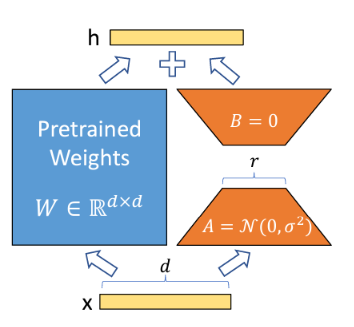
\includegraphics[width=5cm]{fig/lora.png}
\caption{Low-Rank Adaptation (LoRA) applied to a Transformer model.}
\label{fig:lora}
\end{figure}
%\textcolor{red}{TODO} 

\uplevel{\subsection*{Instruction FineTuning}}
%\textcolor{red}{TODO}

As in Homework 1 with the Shakespeare dataset, when given a text, GPT2 (or any LLM for that matter) generates more text to complete the given text. But for a task like text classification, how do you get the model to generate the labels you want for the given context? 

Enter Instruction Fine Tuning. Instruction tuning is a specialized form of fine-tuning in which a model is trained using instruction-output pairs. It helps bridge the gap between the next-word prediction objective of LLMs and the our objective of having LLMs adhere to human instructions.

For the purpose of this homework, you can do this by prepending the text in each sample in the Rotten Tomatoes dataset with an instruction prompt template and then appending it with the actual label. This modified text is what you will train the model with. This happens in the \lstinline{get_sentiment_prompt()} function in \lstinline{dataloader.py}. You can experiment with different instruction templates and ways to respresent the labels.

\uplevel{\subsection*{Implementation}}
Note: In the original paper, LoRA has been implemented only in the attention layers, specifically for the query and value matrices. In this homework you will implement LoRA on the query, key and value matrices.

\textbf{The LoRA Linear Layer:}

\begin{itemize}
    \item In \lstinline{lora.py}, implement these modifications in the \lstinline{LoRALinear} class. This includes:
    \begin{itemize}
        \item \lstinline{__init__}: Initialize inherited nn.Linear class, LoRA parameters, and matrices \(A\) and \(B\) if the LoRA rank is greater than 0.
        \item \lstinline{reset_parameters}: Reinitialize weights of the inherited linear layer and LoRA matrices \(A\) and \(B\). \(A\) is typically initialized with \lstinline{kaiming_uniform_} and \(B\) is initialized with zeroes according to the paper.
        \item \lstinline{forward}: Implement the forward pass of the layer, including the application of LoRA modifications and dropout if applicable.
        \item \lstinline{train}: Override to ensure LoRA matrices are demerged and set to training mode.
        \item \lstinline{eval}: Override to ensure that LoRA matrices are merged with the actual model weight metrices and set to evaluation mode.

    \end{itemize}
        \item \lstinline{mark_only_lora_as_trainable}: A utility function to set only LoRA matrices as trainable parameters for a model. 
\end{itemize}


\textbf{LoRA for Transformer LMs:}
\begin{itemize}
    \item Apply your above implemented LoRALinear layer to the attention layers within your transformer model. This is marked with TODOs in \lstinline{model.py}. 
\end{itemize}

\textbf{Instruction Fine-Tuning Method}
\begin{itemize}
\item All the methods in \lstinline{CustomDataLoader} and \lstinline{dataloader.py} are complete. However, you will return to this file at the end of the empirical section and modify the prompt in \lstinline{get_sentiment_prompt(text, label)}. 
\item Take note of what \lstinline{_add_instruction_finetuning(self, rec)} is doing. \lstinline{rec} is a dataset record with "text" and "label" fields. The function modifies the record by adding an \lstinline{"instr_tuned_text"} field. This field integrates instructional cues into the original text to guide model training. It also converts labels to a more intuitive format (e.g., from numeric to textual labels positive/negative).
\end{itemize}

\textbf{Training:}
\begin{itemize}
    \item Now that you have made your GPT model lora friendly, modify \lstinline{train.py} to enable training with the LoRA-enhanced model. Ensure the model is made LoRA-friendly as indicated by the relevant TODO.
\end{itemize}


\textbf{Accuracy Evaluation Method}

\begin{itemize}
\item In \lstinline{generate.py} you must implement the method \lstinline{predict_labels} which iterates through a dataset, constructs the prompt for each example, and converts the response of the model from a text string to an integer label (1 for positive and 0 for negative).

\item \textbf{Details:} Small models like GPT2 may not easily generate EOS token (especially for small r). Acknowledging these limitations, one simple hack in our case (where training labels are categorical) is to simply check if these labels exists in the first few characters of the generated text. 

\item Make sure that you account for garbage generations when converting from text labels generated by the model to integers. For example, for a given sample, if the model predicts something other than the specified labels(for eg, positive/negative) you should not omit it when calculating accuracy.
\end{itemize}
    
\uplevel{\subsection*{Hints}}
\begin{enumerate}
    \item While implementing your code, you may find it help to adjust the model, e.g. `gpt' is the smallest, but you will need at least `gpt-medium' to see decent results from fine-tuning with LORA.
    \item When trying different variations (across r, alpha, etc) it is recommended you use the \lstinline{--out_dir} flag so you can save the different models you create. 
    \item If you are facing CUDA BLOCKING errors, run with CPU device instead of CUDA on Colab to isolate errors better. Switch to CUDA for the actual training though. 
\end{enumerate}
\clearpage

\uplevel{\subsection*{LoRA Implementation and Training}}
Note: For all the empirical questions report results using gpt2-medium. If not specified, return results using default parameters (i.e with $r=128$, $\alpha=512$, lora\_dropout $=$ \lstinline{0.05}, dropout$=$ \lstinline{0.0}, and learning\_rate $=$ \lstinline{2.5e-4}). Use the default prompt unless mentioned (5.11)
\begin{parts}

\part[2] Does training with LoRA add inference latency (i.e. are more parameters being learned that would add to inference time)? Explain.

\begin{answer_box}[title=,height=3cm, width=15cm]
\end{answer_box}

\part[2] What percentage of parameters are fine-tuned with when you set $r = 128$ and $\alpha = 512$?

\begin{answer_box}[title=,height=3cm, width=15cm]
\end{answer_box}

\uplevel{\subsection*{Inference and Evaluation with LoRA}}
    
\part[1] What is the test accuracy of your model without any fine-tuning? (Hint: you can run this directly using \lstinline{python generate.py --init-from="gpt2-medium"}) [Expected runtime on Colab T4: 2 minutes]

\begin{answer_box}[title=,height=1cm, width=2cm]
\end{answer_box}

\part[4] What is the test accuracy with LoRA fine-tuning across $r \in \{16, 128, 196\}$? What is the test accuracy of full fine-tuning (dropout 0.05) i.e. without LoRA? 
In this question, we maintain a constant scaling factor of 4, i.e. $\alpha = 4r$.  
\emph{Note: In this and all subsequent questions, be sure to report the test accuracy from the ``Best Val Checkpoint'' and \emph{not} the ``Last Iter Checkpoint''.}

[Expected runtime on Colab T4: 25-30 minutes per experiment] 

        \begin{center}
        \renewcommand{\arraystretch}{1.5}
        \begin{tabular}{|c|c|c|p{3cm}|p{5cm}|} 
        \hline
        method & $r$ & alpha & test accuracy (Best Val Checkpoint) \\ \hline
        LoRA & 16 & 64 & \\ \hline 
        LoRA & 128 & 512 & \\ \hline
        LoRA & 196 & 784 & \\ \hline
        Full Fine Tuning (dropout=0.05) & 0 & -- & \\ \hline
        \end{tabular}
        \end{center}


\clearpage
\part[4] Plot wandb validation loss curves for LoRA experiments with \begin{center}
    $(r, \alpha) \in \{(16, 64), (128, 512), (196, 784)\}$ and full fine-tuning ($r=0$).
\end{center}

\begin{answer_box}[title=,height=7cm, width=15cm]
\end{answer_box}

\part[3] How does your fine-tuning with LoRA model's performance compare to full fine-tuning (without LoRA)? Also, how does the value of $r$ affect performance? Briefly discuss (include comments on convergence analysis of validation loss). 

\begin{answer_box}[title=,height=4cm, width=15cm]
\end{answer_box}

\part[2] Is there anything unexpected about the shape of the validation loss when $r=196$? If yes, explain what is unexpected. If no, describe why it appears typical. Do you think it is useful to increase LoRA rank beyond this point $(r=196)$ or should we tune it with different hyperparameters?

\begin{answer_box}[title=,height=3cm, width=15cm]
\end{answer_box}

\clearpage
\part[2] Report the test accuracy and plot wandb validation loss curves for LoRA with $(r, \alpha) \in \{(16, 64), (16, 256)\}$ and full fine-tuning ($r=0$).

[Expected runtime on Colab T4: 25-30 minutes for the new setting] 

\begin{answer_box}[title=,height=10cm, width=15cm]
    \begin{center}
            \renewcommand{\arraystretch}{1.5}
            \begin{tabular}{|c|c|c|c|} 
            \hline
            method & $r$ & alpha & test accuracy (Last Iter Checkpoint) \\ \hline
            LoRA & 16 & 64 & \\ \hline
            LoRA & 16 & 256 & \\ \hline
            Full Fine Tuning (dropout=0.05) & 0 & -- & \\ \hline
            \end{tabular}
    \end{center}
\end{answer_box}


\part[1] In your results from the previous question, how did increasing $\alpha$ while keeping the rank $r$ unchanged affect the performance of the model? Why might this be the case?

\begin{answer_box}[title=,height=4cm, width=15cm]
\end{answer_box}

\part[1] Changing both the learning rate and $\alpha$ may be redundant. Why?

\begin{answer_box}[title=,height=4cm, width=15cm]
\end{answer_box}


\part[1] Modify the variable \lstinline{instruction} in the \lstinline{get_sentiment_prompt()} function within \lstinline{dataloader.py} to experiment with a different prompt during both training and generation. Copy and paste the new instruction here as Python code. Additionally, explain what motivated your choice of modification. You do \emph{not} need to find a prompt that performs better—just explore how changes in phrasing impact the model's behavior.


\begin{tcblisting}{
    listing only,
    listing options={language=Python,breaklines=true,showstringspaces=false},
    height=6cm,
    width=15cm,
    fit,
    enhanced,
    colback=white,
    title=Your Answer,
    sidebyside align=top,
    box align=top,
    title=Code Snippet}
    
    
\end{tcblisting}
\begin{answer_box}[title=Comments,height=3cm, width=15cm]
    
    
\end{answer_box}

\part[2] For the default setting $r = 128, \alpha = 512$, report the test accuracy with the original prompt template and with your new prompt template. (Note that you do \emph{not} need to find one that performs better.)

[Expected runtime on Colab T4: 25-30 minutes for the new setting] 

\begin{answer_box}[title=,height=4cm, width=15cm]
\end{answer_box}

\end{parts}


\clearpage
\sectionquestion{Code Upload}

\begin{parts}

\part[0] Did you upload your code to the appropriate programming slot on Gradescope? \\
\emph{Hint:} The correct answer is `yes'.

    \begin{checkboxes}
     \choice Yes 
     \choice No
    \end{checkboxes}

For this homework, you should upload all the code files that contain your new and/or changed code. Files of type \lstinline{.py} and \lstinline{.ipynb} are both fine.

\end{parts}

\newpage
\sectionquestion{Collaboration Questions}

\begin{parts}

\uplevel{After you have completed all other components of this assignment, report your answers to these questions regarding the collaboration policy. Details of the policy can be found in the syllabus.}

    \part[1] Did you collaborate with anyone on this assignment? If so, list their name or Andrew ID and which problems you worked together on.

        \begin{answer_box}[title=,height=3cm, width=15cm]
        \end{answer_box}

    
    \part[1] Did you find or come across code that implements any part of this assignment? If so, include full details.
        \begin{answer_box}[title=,height=3cm, width=15cm]
        \end{answer_box}
\end{parts}
\end{questions}


\end{document}
